%% Direttive TeXworks:
% !TeX root = ../maltoni_niccolo_tesi.tex
% !TEX encoding = UTF-8 Unicode
% !TEX program = arara
% !TEX TS-program = arara
% !TeX spellcheck = it-IT

\appendix
    % \chapter{Codice relativo all'interfaccia classica}\label{appendix:old}
        % \section{L'interfaccia \texttt{Effect}}\label{appendix:effect}
            % TODO codice

    % \chapter{Codice relativo al contributo}\label{appendix:new}
        % \section{L'interfaccia \texttt{EffectFX}}\label{appendix:effectfx}
            % TODO codice
        \chapter{L'interfaccia \texttt{EffectFX}}\label{appendix:effectfx}
            % TODO UML

        % \section{L'interfaccia \texttt{EffectGroup}}\label{appendix:effectgroup}
            % TODO codice

        %\section{Implementazioni di \texttt{EffectFX} e Proprietà serializzabili}\label{appendix:effectsAndProps}
            % TODO codice
        \chapter{Implementazioni di \texttt{EffectFX} e Proprietà serializzabili}\label{appendix:effectsAndProps}
            % TODO UML
            % \begin{figure}[htbp]
                % \centering
                % 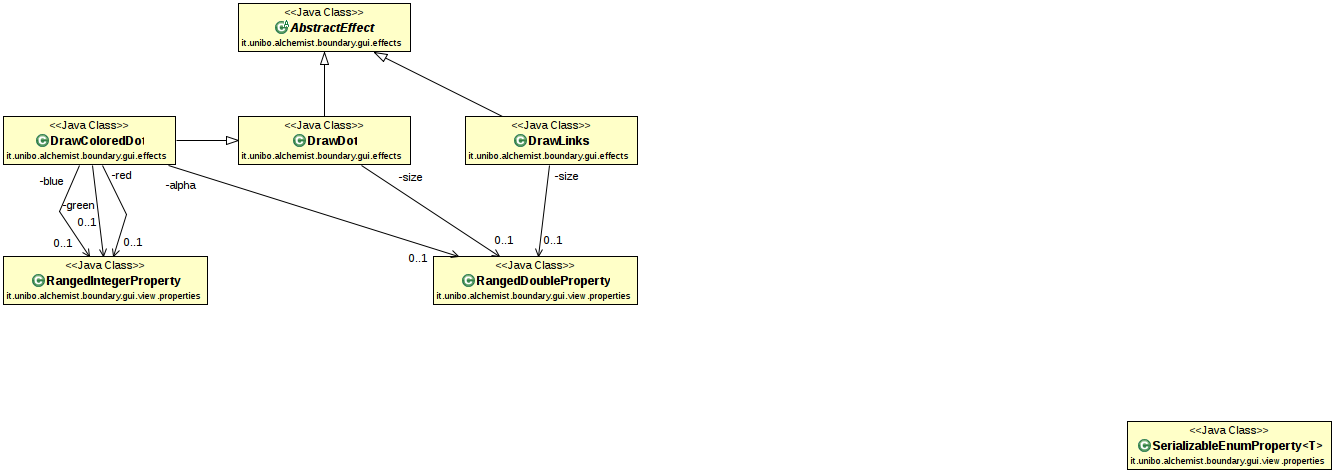
\includegraphics[scale=0.7]{img/EffectAndPropertiesUML}
                % \caption{Il diagramma UML delle classi mostra le relazioni tra gli effetti implementati e le proprietà custom utilizzate}
            % \end{figure}
